 \documentclass[journal,12pt,onecolumn]{IEEEtran}

%--- PREAMBLE ---
% Workaround for conflict between amsmath and txfonts
\let\negmedspace\undefined
\let\negthickspace\undefined

% --- PACKAGES ---
\usepackage[utf8]{inputenc} % Modern input encoding
\usepackage[T1]{fontenc}    % Font encoding for better output
\usepackage{cite}
\usepackage{amsmath,amssymb,amsfonts,amsthm}
\usepackage{algorithmic}
\usepackage{graphicx}
\graphicspath{{./figs/}}
\usepackage{textcomp}
\usepackage{xcolor}
\usepackage{txfonts}
\usepackage{listings}
\usepackage{enumitem}
\usepackage{mathtools}
\usepackage{gensymb}
\usepackage{comment}
\usepackage{caption}
\usepackage{tkz-euclide}
\usepackage{gvv} % Note: This is a non-standard package and requires gvv.sty file
\usepackage{xparse}
\usepackage{array}
\usepackage{longtable}
\usepackage{calc}
\usepackage{multirow}
\usepackage{multicol}
\usepackage{hhline}
\usepackage{ifthen}
\usepackage{lscape}
\usepackage{tabularx}
\usepackage{float}
\usepackage[breaklinks=true]{hyperref} % Should be loaded last

% --- THEOREM DEFINITIONS & CUSTOM COMMANDS ---
\newtheorem{theorem}{Theorem}[section]
\newtheorem{problem}{Problem}
\newtheorem{proposition}{Proposition}[section]
\newtheorem{lemma}{Lemma}[section]
\newtheorem{corollary}[theorem]{Corollary}
\newtheorem{example}{Example}[section]
\newtheorem{definition}[problem]{Definition}
\theoremstyle{remark}

\begin{document}

% --- TITLE & AUTHOR ---
\title{ASSIGNMENT 1: GATE 2010 \\ ME: MECHANICAL ENGINEERING}
\author{EE25BTECH11060 - Namaswi Vajjala}
\maketitle

% Note: The following commands change the numbering of all figures and tables
% to match the main question counter. This can be fragile.
\renewcommand{\thefigure}{\theenumi}
\renewcommand{\thetable}{\theenumi}

% --- MAIN CONTENT ---
\textbf{Q.1-Q.25 carry one mark each}
\begin{enumerate}
    \item  The parabolic arc $y = \sqrt{x},~1 \le x \le 2$ is revolved around the $x$-axis. The volume of the solid of revolution is

    
    \hfill{(GATE ME 2010)}
\begin{multicols}{4}
\begin{enumerate}
\item  $\frac{\pi}{4}$ 
\item $\frac{\pi}{2}$ 
\item $\frac{3\pi}{4}$ 
\item $\frac{3\pi}{2}$
    \end{enumerate}
\end{multicols}
  

\item The Blasius equation,
 \begin{align*}
\frac{d^3f}{d\eta^3} + \frac{f}{2} \frac{d^3f}{d\eta^3}
\end{align*}
=0.\;is a

 \hfill{(GATE ME 2010)}
    \begin{enumerate}
\item second order nonlinear ordinary differential equation 
\item Third order nonlinear ordinary differential equation
\item Third order linear ordinary differential equation
\item Mixed order nonlinear ordinary differential equation
    \end{enumerate}

 
\item The value of the integral is
\begin{align*}
\int_{-1}^{\infty} \frac{dx}{1 + x^2}
\end{align*}

\hfill \text{(GATE ME 2010)}

\begin{multicols}{4}
\begin{enumerate}
    \item $-\pi$
    \item $-\pi/2$
    \item $-\pi/2$
    \item $\pi$
\end{enumerate}
\end{multicols}





\item  The modulus of the complex number ($\frac{3+4i}{1-2i}$) is

 \hfill{(GATE ME 2010)}
 
\begin{multicols}{4}
    \begin{enumerate}

        \item 5
        \item $\sqrt{5}$
        \item $\frac{1}{\sqrt{5}}$
        \item $\frac{1}{5}$
 \end{enumerate}
\end{multicols}


\item The function $y = |2 - 3x|$

 \hfill{(GATE ME 2010)}
 
\begin{enumerate}
\item is continuous $\forall x \in  \mathbb{R}$ and differentiable $\forall x \in \mathbb{R}$
\item is continuous $\forall x \in \mathbb{R}$ and differentiable $\forall x \in \mathbb{R}$ except at $x = \frac{3}{2}$
\item is continuous $\forall x \in \mathbb{R}$ and differentiable $\forall x \in \mathbb{R}$ except at $x = \frac{2}{3}$
\item is continuous $\forall x \in \mathbb{R}$ except at $x = 3$ and differentiable $\forall x \in \mathbb{R}$
\end{enumerate}

 
\item  Mobility of a statically indeterminate structure is 

 \hfill{(GATE ME 2010)}
\begin{multicols}{4}
\begin{enumerate}
\item $\le{-1}$
\item 0
\item 2 
\item $\ge{2}$
\end{enumerate}
\end{multicols}


\item  Then there are 2 points P and Q in a planar body.The relative velocity between 2 points


 \hfill{(GATE ME 2010)}
\begin{enumerate}
\item  should always be along PQ
\item  can be oriented along any direction 
\item  should always be perpendicular to PQ
\item should be along QP when body undergoes pure transition

\end{enumerate}
 

\item The state of plane stress at a point is given by $\sigma_{1}$ = -200MPa  $\sigma_{y}$ = 100MPa $\tau_{xy}$ = 100MPa The maximum sheer stress in(MPa) is 

 \hfill{(GATE ME 2010)}
\begin{multicols}{4}
\begin{enumerate}
\item 111.8
\item 150.1
\item 180.3
\item 223.6
\end{enumerate}
\end{multicols}


\item Which of the following statements is \textbf{INCORRECT}

 \hfill{(GATE ME 2010)}
 
\begin{enumerate}
\item Grashof's rule states that for a planar crank-rocker four bar mechanism, the sum of the shortest and longest link lengths cannot be less than the sum of the remaining  two link lengths.
\item Inversions of a mechanism are created by fixing different links one at a time.
\item Geneva mechanism is an intermittent motion device.
\item Gruebler's criterion assumes mobitity of a planar mechanism to be one
\end{enumerate}
 


\item The natural frequency of a spring mass system on earth is $\omega_{n}$.The natural frequency of the system on moon($g_{moon}$=$\frac{g_{moon}}{6}$) is

 \hfill{(GATE ME 2010)}

 
\begin{multicols}{4}
\begin{enumerate}
\item $\omega_{n}$
\item 0.408$\omega_{n}$
\item 0.204$\omega_{n}$
\item 0.167$\omega_{n}$
\end{enumerate}
\end{multicols}

\item Tooth interference in an external involve spor gear pair can be reduced by

 \hfill{(GATE ME 2010)}

\begin{enumerate}
\item decreasing center distance between gear pair
\item decreasing module 
\item decreasing pressure angle 
\item incraesing number of gear teeth
\end{enumerate}
 

\item For the stability of a floating body,under the influence of gravity alone,which of the following is TRUE?

  \hfill{(GATE ME 2010)}
  
    \begin{enumerate}
        \item Metacentre should be below centre of gravity.
\item Metacentre should be above centre of gravity.
\item Metacentre and centre of gravity must lie on the same horizontal line.
\item Metacentre and centre of gravity must lie on the same vertical line.
    \end{enumerate}
 


\item The maximum velocity of a one-dimensional incompressible fully developed viscous flow, between two fixed parallel plates, is 6 $ms^{-1}$. The mean velocity $\brak{ms^{-1}}$ of the flow is

 \hfill{(GATE ME 2010)}

\begin{multicols}{4}
    \begin{enumerate}
        \item  $2$
        \item $3$
        \item $4$
        \item $5$
    \end{enumerate}
\end{multicols}

\item A phenomenon is modeled using n dimensional variables with k primary dimensions. The number of non-dimensional variables is

 \hfill{(GATE ME 2010)}

\begin{multicols}{4}
    \begin{enumerate}
        \item k
        \item n
        \item n-k
        \item n+k
    \end{enumerate}
\end{multicols}

\item A turbo-charged four-stroke direct injection diesel engine has a displacement volume of 0.0259 m³ $\brak{25.9 liters}$. The engine has an output of 950KW at 2200 rpm. The mean effective pressure $\brak{in\;MPa}$ is closest to

 \hfill{(GATE ME 2010)}
\begin{multicols}{4}
    \begin{enumerate}
        \item $2$
        \item $1$
        \item $0.2$
        \item $0.1$
    \end{enumerate}
\end{multicols}


\item One kilogram of water at room temperature is brought into contact with a high temperature thermal reservoir. The entropy change of the universe is

 \hfill{(GATE ME 2010)}
 
    \begin{enumerate}
        \item equal to entropy change of the reservoir
\item equal to entropy change of water
\item equal to zero
\item always positive
    \end{enumerate}
 

\item A hydraulic turbine develops 1000KW power for a head of 40m. If the head is reduced to 20m, the power developed (in KW )is


 \hfill{(GATE ME 2010)}
 
\begin{multicols}{4}
    \begin{enumerate}
        \item 177
\item 354
\item 500
\item 707
    \end{enumerate}
\end{multicols}

\item The material property which depends only on the basic crystal structure is

 \hfill{(GATE ME 2010)}
 
\begin{multicols}{2}
    \begin{enumerate}
        \item  fatigue strength
\item work hardening
\item  fracture strength
\item  elastic constant
    \end{enumerate}
\end{multicols}

\item In a gating system, the ratio 1:2:4 represents

 \hfill{(GATE ME 2010)}
 
    \begin{enumerate}
        \item  sprue base area: runner area: ingate area
\item pouring basin area: ingate area: runner area
\item sprue base area: ingate area : casting area
\item runner area: ingate area: casting area
    \end{enumerate}
 



\item A shaft has a dimension, $\phi35^{-0.025}$ \; The respective values of fundamental deviation and tolerance are

 \hfill{(GATE ME 2010)}

\begin{multicols}{2}
\begin{enumerate}

\item  -0.025, $\pm{0.08}$

\item  -0.025, 0.016

\item -0.009, $\pm{0.008}$

\item  -0.009, 0.016
 \end{enumerate}
\end{multicols}

\item In a CNC program block, N002 G02 G91 X40 ZA0  , G02 and G91 refer to

  \hfill{(GATE ME 2010)}
  
\begin{enumerate}

    \item circular interpolation in counterclockwise direction and incremental dimension
    \item  circular interpolation in counterclockwise direction and absolute dimension
    \item circular interpolation in clockwise direction and incremental dimension
    \item circular interpolation in clockwise direction and absolute dimension
    \end{enumerate}
 


\item The demand and forecast for February are 12000 and 10275, respectively. using single exponential smoothening method $\brak{smoothening\;coefficient = 0.25}$, forecast for the month of March is

 \hfill{(GATE ME 2010)}
 
\begin{multicols}{4}
\begin{enumerate}

\item 431
\item 9587
\item 10706
\item 11000
 \end{enumerate}
\end{multicols}



\item Little's law is a relationship between

  \hfill{(GATE ME 2010)}
  
\begin{enumerate}

\item stock level and lead time in an inventory system
\item waiting time and length of the queue in a queuing system
\item number of machines and job due dates in a scheduling problem
\item uncertainty in the activity time and project completion time
\end{enumerate}
 


\item vechile manufacturing assembly line is an example of

  \hfill{(GATE ME 2010)}
  
\begin{multicols}{2}
    \begin{enumerate}
        \item product layot
        \item process layot
        \item manufacture layot
        \item fixed layot
    \end{enumerate}
\end{multicols}


\item Simplex method of solving linear programming problem uses

  \hfill{(GATE ME 2010)}
 
    \begin{enumerate}

\item all the points in the feasible region
\item  only the comer points of the feasible region
\item  intermediate points within the infeasible region
\item  only the interior points in the feasible region
  \end{enumerate}
 

\textbf{Q.26-Q.55 carry two marks each }

\item Torque exerted on a flywheel over a cycle is listed in the table. Flywheel energy $\brak{in J per unit cycle}$ using Simpson's rule is 
\[
\begin{array}{|c|c|c|c|c|c|c|c|c|}
\hline
\text{Angle (degree)} & 0 & 60 & 120 & 180 & 240 & 300 & 360 \\
\hline
\text{Torque (N\,m)} & 0 & 1066 & -323 & 0 & 323 & -355 & 0 \\
\hline
\end{array}
\]

  \hfill{(GATE ME 2010)}


\begin{multicols}{4}
\begin{enumerate}
    
    \item 542
    \item 993
    \item 1444
    \item 1983
\end{enumerate}
\end{multicols}


 \item One of the eigenvectors of the matrix
\( A = \begin{bmatrix} 2 & 2 \\ 1 & 3 \end{bmatrix} \) is

\hfill{(GATE ME 2010)}
\begin{multicols}{4}
\begin{enumerate}
    \item \( \myvec{2 \\ -1} \)
    \item \( \myvec{2 \\ 1} \)
    \item \( \myvec{4 \\ 1} \)
    \item \( \myvec{1 \\ -1} \)
\end{enumerate}
\end{multicols}



\item Velocity vector of a flow field is given as  \myvec{V} =$2xy\,\hat{i} - x^2\,\hat{j}$.
The velocity vector at $\brak{1,1,1}$ is

  \hfill{(GATE ME 2010)}

\begin{multicols}{2}
\begin{enumerate}
    \item $4\hat{i}-\hat{j}$
    \item $4\hat{i}-\hat{k}$
    \item $\hat{i}-4\hat{j}$
    \item $\hat{i}-4\hat{j}$
\end{enumerate}
\end{multicols}


\item The Laplace transform of a function $f(t)$ is $\frac{1}{(s^{2})(s+1)}$.The function $f(t)$ is

  \hfill{(GATE ME 2010)}
  
\begin{multicols}{4}
\begin{enumerate}

\item t-1+$e^{t}$
\item t+1+$e^{-t}$
\item -1+$e^{-t}$
\item 2t+$e^{-t}$
\end{enumerate}
\end{multicols}


\item A box contains 2 washers, 3 nuts and 4 bolis. Items are drawn from the box at random one at a time without replacement. The probability of drawing 2 washers first followed by 3 nuts and subsequently the 4 bolis is

  \hfill{(GATE ME 2010)}
  
\begin{multicols}{4}
\begin{enumerate}
\item $\frac{2}{315}$
\item $\frac{1}{630}$
\item $\frac{1}{1260}$
\item $\frac{1}{2520}$

\end{enumerate}
\end{multicols}


\item A band brake having band-width of 80 mm, drum diameter of 250 mm, coefficient of friction of 0.25 and angle of wrap of 270 degrees is required to exert a friction torque of 1000 N m. The maximum tension $\brak{in\;kN}$developed in the band is

  \hfill{(GATE ME 2010)}
  
\begin{multicols}{4}
\begin{enumerate}
\item 1.88
\item 3.56
\item 6.12
\item 11.56
\end{enumerate}
\end{multicols}


\item A bracket $\brak{shown\ in\ figure}$ is rigidly mounted on wall using four rivets. Each rivet is 6mm in diameter and has an effective length of 12mm.
 
 \begin{figure}[H]
    \centering
    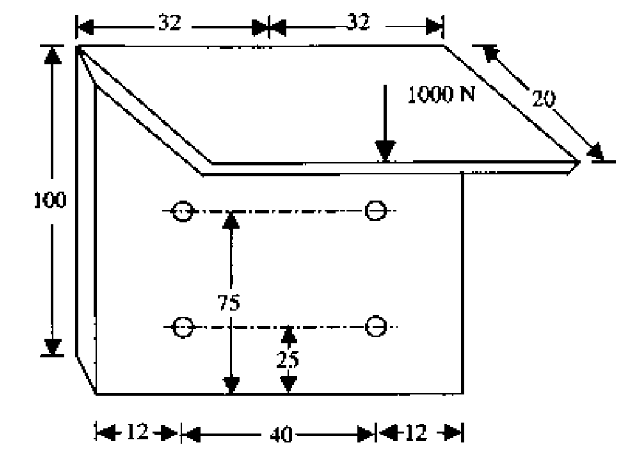
\includegraphics[width=0.7\columnwidth]{figs/fig1.png}
    \caption*{}
    \label{fig:Q32}
\end{figure}


Direct shear stress $\brak{in\;MPa}$ in the most heavily loaded rivet is 


  \hfill{(GATE ME 2010)}

\begin{multicols}{4}
\begin{enumerate}
\item 4.4
\item 8.8
\item 17.6
\item 35.2
\end{enumerate}
\end{multicols}



\item A mass m attached to a spring is subjected to a harmonic force as shown in figure. The amplitude of the forced motion is observed to be 50 mm. The value of m (in kg) is
 \begin{figure}[H]
    \centering
    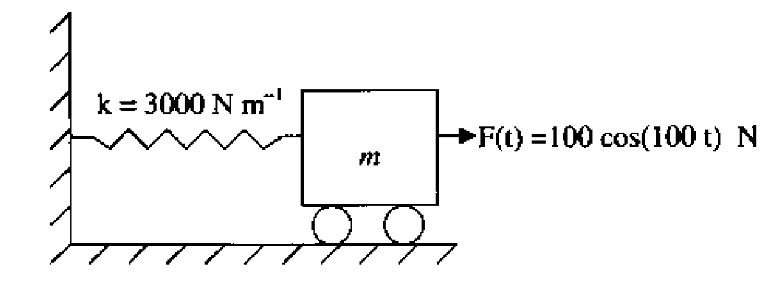
\includegraphics[width=0.7\columnwidth]{figs/fig2.png}
    \caption*{}
    \label{fig:Q33}
\end{figure}


\hfill{(GATE  ME 2010)}


\begin{multicols}{4}
\begin{enumerate}
\item 0.1
\item 1.0
\item 0.3
\item 0.5
\end{enumerate}
\end{multicols}

\item For the epicyclic gear arrangement shown in the figure, $w_{2}=100$ clockwise $\brak{CW}$ and $w_{arod}$= 80 rad/s counter clockwise $\brak{CCW}$. The angular velocity $\brak{in\;rad/s}$ is


\hfill{(GATE  ME 2010)}

 \begin{figure}[H]
    \centering
    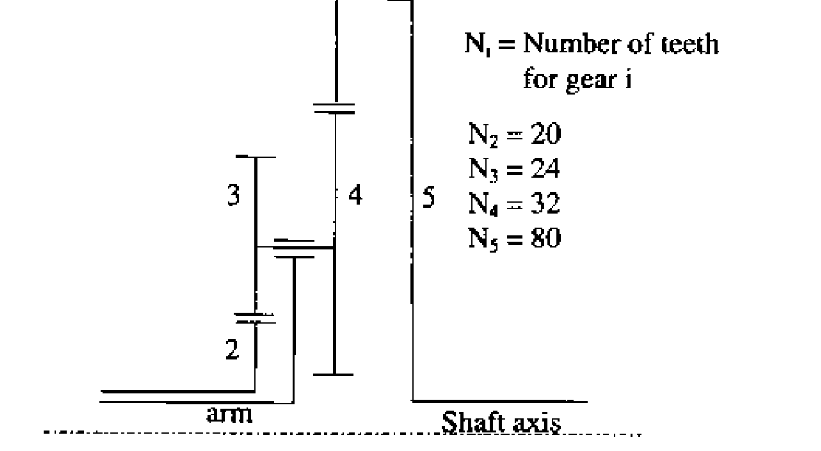
\includegraphics[width=0.7\columnwidth]{figs/fig3.png}
    \caption*{}
    \label{fig:Q34}
\end{figure}

\begin{multicols}{4}
\begin{enumerate}
\item 0
\item 70CW
\item 140CCW
\item 140CW
\end{enumerate}
\end{multicols}


\item  A lightly loaded full journal bearing has journal diameter of 50 mm, bush bore of 50.05 mm and bush length of 20 mm. If rotational speed of journal is 1200 rpm and average viscosity of liquid lubricant is 0.03 Pa s. the power loss (in W) will be

\hfill{(GATE  ME 2010)}

\begin{multicols}{4}
\begin{enumerate}
    \item 37
    \item 74
    \item 118
    \item 237
\end{enumerate}
\end{multicols}

\item For the configuration shown, the angular velocity of link AB is 10 rad/s countorclockwise. The magnitude of the relative sliding velocity (in ms"') of slider B with respect to rigid link CD is
 \begin{figure}[H]
    \centering
    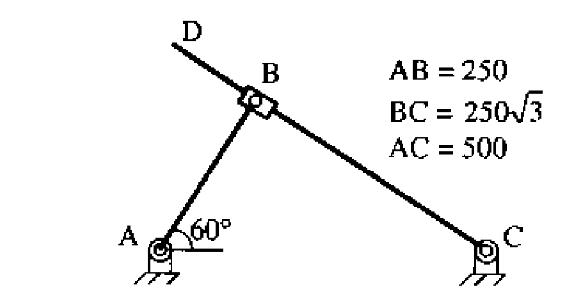
\includegraphics[width=0.7\columnwidth]{figs/fig4.png}
    \caption*{}
    \label{fig:Q36}
\end{figure}



\hfill{(GATE  ME 2010)}


\begin{multicols}{4}
\begin{enumerate}
\item 0
\item 0.86
\item 1.25
\item 0.25
\end{enumerate}
\end{multicols}


\item A smooth pipe of diameter 200 mm carries water. The pressure in the pipe at section SI (elevation:10m ) is 50 kPa . At section S2 (elevation: 12m ) the pressure is 20 kPa and velocity is 2 $ms^{-1}$
Density of water is 1000  $kgm^{-3}$ and acceleration due to gravity is $9.8 ms^{-2}$  Which of the  following is TRUE


\hfill{(GATE  ME 2010)}

\begin{enumerate}
\item  flow is from S1 to S2 and head toss is 0.53 m
\item  flow is from S2 to S1 and head loss is 0.53 m
\item  flow is from SI to S2 and head loss is 1.06 m
\item  flow is from S2 to SI and head loss is 1.06 m
\end{enumerate}


\item  Match the following 

 $
\begin{array}{|l|l|}
\hline
\text{P: Compressible flow} & \text{U: Reynolds number} \\ \hline
\text{Q: Free surface flow} & \text{V: Nusselt number} \\ \hline
\text{R: Boundary layer flow} & \text{W: Weber number} \\ \hline
\text{S: Pipe flow} & \text{X: Froude number} \\ \hline
\text{T: Heat convection} & \text{Y: Mach number} \\ \hline
& \text{Z: Skin friction coefficient} \\ \hline
\end{array}
$


\hfill{(GATE  ME 2010)}




\begin{multicols}{2}
\begin{enumerate}
\item P-U; Q-X; R-V; S-Z; T-W
\item P-W; Q-X; R-Z: S-U; T-V
\item P-Y: Q-W: R-Z: S-U: T-X
\item P-Y; Q-W; R-Z: S-U; T-V
\end{enumerate}
\end{multicols}

\item A mono-atomic ideal gas (y=1.67, molecular weight = 40) is compressed adiabatically from 0.1 MPa, 300K to 0.2 MPa. The universal gas constant is 8.314 kJ kmol"' K-1. The work of compression of the gas (in kJ kg"' ) is


\hfill{(GATE  ME 2010)}


\begin{multicols}{4}
\begin{enumerate}
\item 29.7
\item 19.9
\item 13.3
\item 0
\end{enumerate}
\end{multicols}


\item Consider the following two processes;
a. A heat source at 1200K loses 2500kJ of heat to a sink al 800K
b. A heat souree at 800K loses 2000kJ of heat to a sink at 500K
Which of the following statements is true?

\hfill{(GATE  ME 2010)}

 
\begin{enumerate}
\item Process I is more irreversible than Process II
\item Process II is more irreversible than Process I
\item Icreversibility associated in both the processes are equal
\item Both the processes are reversible
\end{enumerate}
 


\item A fin has 5 mm diameter and 100 mm length. The thermal conductivity of fin material is
400Wm-'K-1, One end of the fin is maintained at 130℃ and its remaining surface is exposed to
ambient air at 30C. If the convective heat transfer coefficient is 40Wm- K-', the heal loss
(in W) from the fin is

\hfill{(GATE  ME 2010)}


\begin{multicols}{4}
\begin{enumerate}
\item 0.08
\item 5.00
\item 7.00
\item 7.80
\end{enumerate}
\end{multicols}

\item A inoist air sample has dry bulb temperature of 30℃ and specific humidity of 11.5 g water vapour per kg dry ajr. Assume molecular weight of air as 28.93. If the saturation vapour pressure of water at 30"C is 4.24 kPa and the total pressure is 90 kPa, then the relative humidity (in %) of air
sample is


\hfill{(GATE  ME 2010)}


\begin{multicols}{4}
\begin{enumerate}
\item 50.5
\item 38.5
\item 56.5
\item 68.5
\end{enumerate}
\end{multicols}


\item Two pipes of inner diamerer 100 mm and outer diameter 110 mm each are joined by nlash-butz welding using 30 V power supply. At the interface, 1 mm of malcrial melts from each pipe which bas a resistance of 42.4Q. If the unit melt energy is 64.4MJ m"1, then time required for welding (in s) is

\hfill{(GATE  ME 2010)}


\begin{multicols}{4}
\begin{enumerate}
\item 1
\item 5
\item 10
\item 20
\end{enumerate}
\end{multicols}

\item For tool A, Taylor's tool life exponent $\brak{n}$ is 0.45 and constant $\brak{K}$ is 90. Similarly for tool B, n = 0.3 and K= 60. The cutting speed $\brak{inm/min}$ above which tool A will have a higher tool life than tool B is

\hfill{(GATE  ME 2010)}\\

\begin{multicols}{4}
\begin{enumerate}
\item 26.7
\item 42.5
\item 80.7
\item 142.9
\end{enumerate}
\end{multicols}

\item A taper hole is inspected using a CMM, with a probe of 2 mm diameter. At a height, Z = 10 mm from the bottom, 5 points are touched and a diameter of circle $\brak{not\;compensated\;for\;size}$ is obtained as 20 mm. Similarly, a 40 mm diameter is obtained at a height Z = 40 mm. The smaller diameter $\brak{in mm}$ of hole at Z = 0 is


\hfill{(GATE  ME 2010)}

  \begin{figure}[H]
    \centering
    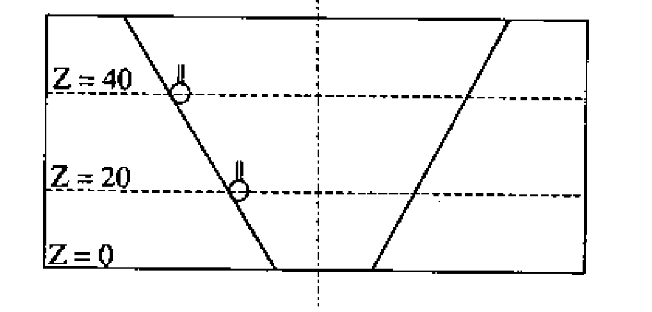
\includegraphics[width=0.7\columnwidth]{figs/fig5.png}
    \caption*{}
    \label{fig:Q45}
\end{figure}

\begin{multicols}{4}
\begin{enumerate}
\item 13.334
\item 15.334
\item 15.442
\item 15.542
\end{enumerate}
\end{multicols}


\item  Annual demand for window frames is 10000. Each frame costs Rs. 200 and ordering cost is Rs. 300 per order. Inventory holding cost is Rs. 40 per frame per year. The supplier is willing to offer 2% discount if the order quantity is 1000 or more, and 4% if order quantity is 2000 or more. If the total cost is to be minimized, the retailer should

\hfill{(GATE  ME 2010)}


\begin{enumerate}
\item  order 200 frames every time
\item  accept 2% discount
\item  accept 4% discount
\item order Economic Order Quantity
\end{enumerate}


\item The project activities, precedence relationships and durations are described in the table. The critical path of the project is
\[
\begin{array}{|c|c|c|}
\hline
\text{Activity} & \text{Precedence} & \text{Duration (in days)} \\
\hline
P & - & 3 \\
Q & - & 4 \\
R & P & 5 \\
S & Q & 5 \\
T & R, S & 7 \\
U & R, S & 5 \\
V & T & 2 \\
W & U & 10 \\
\hline
\end{array}
\]


 \hfill{(GATE  ME 2010)}\\


\begin{multicols}{2}
\begin{enumerate}
\item P-R-T-V
\item  Q-S-T-Y
\item P-R-U-W
\item Q-S-U-W
\end{enumerate}
\end{multicols}
\hfill{(GATE ME 2010)}\\
\textbf{Common Data Questions}

\textbf{Common Data for Questions 48 and 49}

In a steam power plant operating on the Rankine cycle, steam enters the turbine at 4MPa, 350 C and exits at a pressure of 15 kPa. Then it enters the condenser and exits as saturated water. Next, a pump feeds back the water to the boiler. The adiabatic efficiency of the turbine is 90\%. The thermodynamic states of water and steam are given in the table.


 \begin{table}[ht]
\centering
\begin{tabular}{|l|c|c|c|}
\hline
\textbf{State} & \textbf{$h$ (kJ/kg)} & \textbf{$s$ (kJ/kg·K)} & \textbf{$\nu$ (m³/kg)} \\
\hline
Steam: 4 MPa, 350°C & 3092.5 & 6.5821 & 0.06645 \\
\hline
Water: 15 kPa & $h_f = 225.94$ & $s_f = 0.7549$ & $v_f = 0.001014$ \\
               & $h_g = 2599.1$ & $s_g = 8.0085$ & $v_g = 10.02$ \\
\hline
\end{tabular}
\caption{Thermodynamic properties of steam and water at specified states.}
\label{tab:steam_water}
\end{table}





h is specific enthalpy, s is specific entropy and v the specific volume; subscripts f and g denote saturated
liquid state and saturated vapour state.
\item The network $(KJ Kg^{-1})$ output of the cycle


\hfill{(GATE  ME 2010)}\\

\begin{multicols}{4}
\begin{enumerate}
\item 498
\item 775
\item 860
\item 957
\end{enumerate}
\end{multicols}


\item Heat supplied $(kJkg^{-1})$ to the cycle is

\hfill{(GATE  ME 2010)}\\


\begin{multicols}{4}
\begin{enumerate}
\item 2372
\item 2576
\item 2863
\item 3092
\end{enumerate}
\end{multicols}



\textbf{Common Data for Questions 50 and 51:}

Four jobs are to be processed on a machine as per data listed in the table
\begin{table}[h!]
  \centering
  \begin{tabular}{|c|c|c|}
    \hline
    \textbf{Job} & \textbf{Processing limit (in days)} & \textbf{Due date} \\
    \hline
    1 & 4 & 6 \\
    \hline
    2 & 7 & 9 \\
    \hline
    3 & 2 & 19 \\
    \hline
    4 & 8 & 17 \\
    \hline
  \end{tabular}
  \caption*{}
  \label{tab:jobs}
\end{table}

\item If the Earliest Due Date $\brak{EED}$ rule is used to sequence the jobs, the number of jobs delayed is


\hfill{(GATE  ME 2010)}\\


\begin{multicols}{4}
\begin{enumerate}
\item 1
\item 2
\item 3
\item 4
\end{enumerate}
\end{multicols}


\item Using the Shortest Processing Time (SPT) rule, 1o1al tardiness is

\hfill{(GATE  ME 2010)}\\

\begin{multicols}{4}
\begin{enumerate}
\item 0
\item 2
\item 6
\item 8
\end{enumerate}
\end{multicols}


\textbf{Linked Answer Questions
Statement for Linked Answer Questions 52 and 53:}\\

 A massless beam has a loading pattern as shown in the figure. The beam is of rectangular cross-section with a width of 30 mm and height of 100 mm.
 \begin{figure}[H]
    \centering
    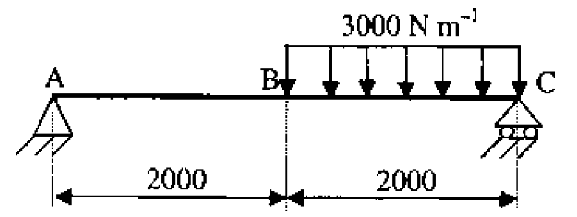
\includegraphics[width=0.7\columnwidth]{figs/fig6.png}
    \caption*{}
    \label{fig:Q51}
\end{figure}


\item The maximum bending moment occurs at 



 \hfill{(GATE  ME 2010)}\\

\begin{enumerate}
\item Location B
\item 2675 mm lo the right of A
\item 2500 mm to the right of A
\item 3225 mm to the right of A
\end{enumerate}


\item The maximum magnitude of bending stress (in MPa) is given by

\hfill{(GATE  ME 2010)}\\


\begin{multicols}{4}
\begin{enumerate}
\item 60.0
\item 67.5
\item 200.0
\item 225.0
\end{enumerate}
\end{multicols}

\textbf{Statement for Linked Answer Questions 54 and 55:}\\

 In shear cutting operation, a sheet of 5 mm thickness is cut along a length of 200 mm. The cutting blade is 400 mm long (see figure) and zero-shear (S = 0) is provided on the edge. The ultimate shear strength of the sheet is 100 MPa and penetration to thickness ratio is 0.2. Neglect friction.
 \begin{figure}[H]
    \centering
    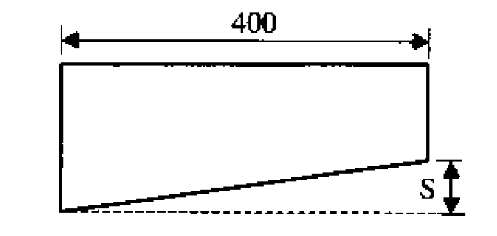
\includegraphics[width=0.7\columnwidth]{figs/fig7.png}
    \caption*{}
    \label{fig:Q54}
\end{figure}

 \item Assuming force vs displacement curve is regular then the work done is 


 \hfill{(GATE  ME 2010)}\\

\begin{multicols}{4}
\begin{enumerate}
\item 100
\item 200
\item 250
\item 300
\end{enumerate}
\end{multicols}

\item A shear of 20 mm (S = 20 mm) is now provided on the blade. Assuming force vs displacement curve to be trapezoidal, the maximum force (in kN) exerted is

\hfill{(GATE  ME 2010)}\\


\begin{multicols}{4}
\begin{enumerate}
\item 5
\item 10 
\item 20
\item 40
\end{enumerate}
\end{multicols}

\textbf{General Aptitude (GA) Questions
Q.56 - Q.60 carry one mark each.}\\

\item 25 persons are in a room. 15 of them play hockey, 17 of them play football and 10 of them play both hockey and football. Then the number of persons playing neither hockey nor football is:

\hfill{(GATE  ME 2010)}\\


\begin{multicols}{4}
\begin{enumerate}
\item 2
\item 17
\item 13
\item 3
\end{enumerate}
\end{multicols}



\item \textit{Choose the most appropriate word from the options given below to complete the following sentence:}
\textbf{If we manage to our natural resources,we would live a better planet for our  children.}


\hfill{(GATE  ME 2010)}\\

\begin{multicols}{4}
\begin{enumerate}
\item uphold
\item restrain
\item cherish
\item conserve
\end{enumerate}
\end{multicols}



\item \textit{The question below consists of a pair of related words followed by four pairs of words. Select the pair that best expresses the relation in the original pair.}
\textbf{Unemployed : Worker}

\hfill{(GATE  ME 2010)}\\


\begin{enumerate}
\item fallow : land
\item unaware : sleeper
\item wit : jester
\item renovated : house
\end{enumerate}



\item Which of the following options is the closest in meaning to the word below:
\textbf{Circuitous}


\hfill{(GATE  ME 2010)}\\

\begin{enumerate}

\item cyclie
\item indirect
\item confusing
\item crooked
\end{enumerate}


\item Choose the most uppropriate word from the oprions given below to complete the following
sentence:
\textbf{His rather casual remarks on politics bis lack of seriousness about the subject.}

\hfill{(GATE  ME 2010)}\\


\begin{multicols}{4}
\begin{enumerate}

\item  masked
\item  belied
\item  betrayed
\item  suppressed
\end{enumerate}
\end{multicols}



\textbf{ Q.61 -Q.65 carry two marks each.}\\
\item  Hari (H), Gita (G), Irfan (I) and Saira (S) are siblings (i.e. brothers and sisters). All were born on
1" January. The age difference between any two successive siblings (that is born one after another)
is less than 3 years. Given the following facls:\\
i. Hari's age + Gita's age > Irfan's age + Saira's age.\\
ii. The age difference between Gita and Saira is 1 year. However, Gita is not the
oldest and Saira is not the youngest.\\
iii. There are no twins.
In what order were they born (oldest first)?
\begin{enumerate}

\item SGEI
\item  HSIG
\item IGSH
\item IHSG
\end{enumerate}


\item 5 skilled workers can build a wall in 20 days; 8 semi-skilled workers can build a wall in 25 days;
10 unskilled workers can build a wall in 30 days. If a team has 2 skilled, 6 semi-skilled and
5 unskilled workers. how long will it take to build the wall?

\hfill{(GATE  ME 2010)}\\

\begin{multicols}{4}
\begin{enumerate}

\item 20 days
\item 18 days
\item 16 days
\item 15 days
\end{enumerate}
\end{multicols}



\item \textbf{Modern warfare has changed from large scale clashes of armies to suppressioo of civilian
populations. Chemical agents that do their work silently appear to be suited to such warfare;
and regretfully, there exist people in military establishments who think that chemical agents
are useful tools for their cause.}

Which of the following statements best sums up the meaning of the above passage:

\hfill{(GATE  ME 2010)}\\

\begin{enumerate}
\item Modem warfare has resulted in civil strife.
\item  Chemical agents are useful in modern warfare.
\item  Use of chemical agents in warfare would be undesirable.
\item  People in military establishments like to use chemical agents in war.
\end{enumerate}


\item Given digits 2, 2. 3, 3, 3, 4, 4, 4, 4 how many distinct 4 digit numbers greater than 3000 can be
formed?

\hfill{(GATE  ME 2010)}\\

\begin{multicols}{4}
\begin{enumerate}
    \item 50
    \item 51
    \item 52
    \item 54
\end{enumerate}
\end{multicols}
\item If 137+276=435 how much is 731+672?

\hfill{(GATE  ME 2010)}\\

\begin{multicols}{4}
\begin{enumerate}
    \item 534
    \item 1403
    \item 1623
    \item  1513
\end{enumerate}
\end{multicols}
\end{enumerate}
\end{document}